\documentclass[12pt,a4paper]{article}

% -------------------------------------------------
% Packages
% -------------------------------------------------
\usepackage[a4paper,margin=1in]{geometry}
\usepackage{amsmath,amssymb,amsthm}
\usepackage{tikz}
\usetikzlibrary{positioning,calc}
\usepackage{enumitem}
\usepackage{graphicx}
\usepackage{hyperref}
\usepackage{fancyhdr}

% -------------------------------------------------
% Page Style
% -------------------------------------------------
\pagestyle{fancy}
\fancyhf{}
\lhead{Mathematics for Computing(MFC)}
\rhead{Set Theory}
\cfoot{\thepage}

% -------------------------------------------------
% Hyperlink Settings
% -------------------------------------------------
\hypersetup{
    colorlinks=true,
    linkcolor=black,
    urlcolor=blue
}

% -------------------------------------------------
% Document
% -------------------------------------------------
\begin{document}

% =================================================
% TITLE PAGE
% =================================================

\begin{titlepage}
\centering

\vspace*{1.2cm}

{\Large \textbf{COCHIN UNIVERSITY OF SCIENCE AND TECHNOLOGY}}

\vspace{0.4cm}

{\large \textbf{Dept. of Computer Science}}

\vspace{1.5cm}

{\Large \textbf{MATHEMATICS FOR COMPUTING(MFC)}}

\vspace{1cm}

{\Huge \textbf{SET THEORY}}

\vspace{1.2cm}

{\large Assignment}

\vfill

\begin{center}
\textbf{Pranav M P}

\vspace{0.25cm}

Reg. No: 24102366 (S5,Y3)

\vspace{0.25cm}

Int. M.Sc CS

\vspace{0.25cm}

Dept. of Computer Science

\vspace{0.25cm}

CUSAT
\end{center}

\vfill

{\large \today}

\end{titlepage}

% =================================================
% TABLE OF CONTENTS
% =================================================

\tableofcontents

\newpage

% =================================================
% INTRODUCTION
% =================================================

\section{Introduction}

Set theory is one of the fundamental branches of mathematics and forms the basis
of many concepts in computer science, logic, probability, and discrete mathematics.
A set is a well-defined collection of distinct objects called elements. Sets are
usually represented by capital letters, while their elements are enclosed within
curly braces.

For example,

\[
A=\{1,2,3,4,5\}
\]

Here, $1,2,3,4$ and $5$ are the elements of $A$.

The symbol $\in$ means ``belongs to''. Therefore,

\[
3\in A
\]

while

\[
7\notin A.
\]

% =================================================
% TYPES AND REPRESENTATION OF SETS
% =================================================

\section{Types and Representation of Sets}

% -------------------------------------------------

\subsection{Cardinality of a Set}

The cardinality of a set is the total number of elements present in the set.
It is denoted by

\[
|A|.
\]

For example, if

\[
A=\{2,4,6,8\},
\]

then

\[
|A|=4.
\]

Therefore, the cardinality of $A$ is 4.

% -------------------------------------------------

\subsection{Finite Set}

A finite set contains a limited number of elements.

For example,

\[
A=\{a,b,c,d\}.
\]

Since there are only four elements,

\[
|A|=4.
\]

Therefore, $A$ is a finite set.

% -------------------------------------------------

\subsection{Infinite Set}

An infinite set contains infinitely many elements.

For example,

\[
\mathbb{N}=\{1,2,3,4,\ldots\}.
\]

The set of natural numbers continues indefinitely. Hence, it is an infinite set.

% -------------------------------------------------

\subsection{Empty (Null) Set}

A set containing no elements is called an empty or null set.

It is represented by

\[
\emptyset
\]

or

\[
\{\}.
\]

For example, the set of natural numbers less than zero is

\[
\emptyset.
\]

The cardinality of an empty set is

\[
|\emptyset|=0.
\]

% -------------------------------------------------

\subsection{Singleton Set}

A singleton set contains exactly one element.

For example,

\[
A=\{5\}.
\]

Here,

\[
|A|=1.
\]

Therefore, $A$ is a singleton set.

% -------------------------------------------------

\subsection{Equal Sets}

Two sets are equal if they contain exactly the same elements.

For example,

\[
A=\{1,2,3\}
\]

and

\[
B=\{3,2,1\}.
\]

Although the order is different,

\[
A=B.
\]

The order of elements does not affect a set.

% -------------------------------------------------

\subsection{Equivalent Sets}

Two sets are called equivalent if they contain the same number of elements.

For example,

\[
A=\{1,2,3\}
\]

and

\[
B=\{a,b,c\}.
\]

Since

\[
|A|=|B|=3,
\]

the two sets are equivalent.

% -------------------------------------------------

\subsection{Unique Set}

A set contains only distinct elements. Repeated elements are not considered
separate elements.

For example,

\[
\{1,2,2,3,3,3\}
=
\{1,2,3\}.
\]

Therefore,

\[
|\{1,2,2,3,3,3\}|=3.
\]

% -------------------------------------------------

\subsection{Set-Builder Form}

A set can be represented by describing a property or condition that all
its elements satisfy. This method of representing a set is called the
\textbf{set-builder form}.

It is generally written as

\[
A=\{x\mid P(x)\},
\]

where $x$ represents an element and $P(x)$ is the condition that the
element must satisfy. The symbol ``$\mid$'' is read as ``such that''.
A colon ``:'' can also be used instead of ``$\mid$''.

\textbf{Example:}

The set of even natural numbers less than 10 can be written in roster
form as

\[
A=\{2,4,6,8\}.
\]

In set-builder form,

\[
A=\{x\in\mathbb{N}\mid x<10\text{ and }x\text{ is even}\}.
\]

Another example is

\[
B=\{x\in\mathbb{Z}\mid -2\leq x\leq2\}.
\]

In roster form, this set is

\[
B=\{-2,-1,0,1,2\}.
\]

Thus, the set-builder form describes a set by specifying the condition
satisfied by its elements.

% -------------------------------------------------

\subsection{Complete Set}

A complete set contains all the elements being considered in a particular
context. This idea is commonly represented using the universal set.

For example, if the numbers from 1 to 10 are being considered,

\[
U=\{1,2,3,4,5,6,7,8,9,10\}.
\]

If

\[
A=\{2,4,6\},
\]

then every element of $A$ belongs to the complete set $U$.

% -------------------------------------------------

\subsection{Subset}

A set $A$ is called a subset of $B$ if every element of $A$ is also an element
of $B$.

It is written as

\[
A\subseteq B.
\]

Formally,

\[
A\subseteq B
\iff
(\forall x)(x\in A\Rightarrow x\in B).
\]

For example,

\[
A=\{1,2\}
\]

and

\[
B=\{1,2,3,4\}.
\]

Hence,

\[
A\subseteq B.
\]

% -------------------------------------------------

\subsection{Proper Subset}

If

\[
A\subseteq B
\]

and

\[
A\neq B,
\]

then $A$ is called a proper subset of $B$.

It is written as

\[
A\subset B.
\]

For example,

\[
A=\{1,2\}
\]

and

\[
B=\{1,2,3\}.
\]

Therefore,

\[
A\subset B.
\]

% -------------------------------------------------

\subsection{Superset}

If

\[
A\subseteq B,
\]

then $B$ is called a superset of $A$.

It is written as

\[
B\supseteq A.
\]

For example,

\[
B=\{1,2,3,4\}
\]

and

\[
A=\{1,2\}.
\]

Therefore,

\[
B\supseteq A.
\]

% -------------------------------------------------

\subsection{Universal Set}

The universal set contains all the elements under consideration. It is usually
denoted by $U$.

For example,

\[
U=\{1,2,3,4,5,6,7,8,9,10\}
\]

and

\[
A=\{2,4,6\}.
\]

Since every element of $A$ belongs to $U$,

\[
A\subseteq U.
\]

% -------------------------------------------------

\subsection{Power Set}

The power set of a set is the set of all possible subsets of that set.

It is denoted by

\[
\mathcal{P}(A).
\]

If a set contains $n$ elements, its power set contains

\[
2^n
\]

subsets.

For example, let

\[
A=\{a,b\}.
\]

Then

\[
\mathcal{P}(A)
=
\{\emptyset,\{a\},\{b\},\{a,b\}\}.
\]

Since

\[
|A|=2,
\]

we have

\[
|\mathcal{P}(A)|=2^2=4.
\]

% -------------------------------------------------

\subsection{Countable Set}

A set whose elements can be counted one by one is called a countable set.

For example,

\[
\mathbb{N}=\{1,2,3,\ldots\}
\]

is a countably infinite set.

The sets of integers $\mathbb{Z}$ and rational numbers $\mathbb{Q}$
are also countable.

% -------------------------------------------------

\subsection{Uncountable Set}

A set that cannot be put into one-to-one correspondence with the natural
numbers is called an uncountable set.

For example, the set of real numbers

\[
\mathbb{R}
\]

is uncountable.

% =================================================
% OPERATIONS ON SETS
% =================================================

\section{Operations on Sets}

Let

\[
A=\{1,2,3,4\}
\]

and

\[
B=\{3,4,5,6\}.
\]

The following operations use these sets as common examples.

% -------------------------------------------------

\subsection{Union of Sets}

The union of two sets contains every element that belongs to either set
or to both sets.

It is denoted by

\[
A\cup B.
\]

Mathematically,

\[
A\cup B
=
\{x\mid x\in A\text{ or }x\in B\}.
\]

For the given sets,

\[
A\cup B=\{1,2,3,4,5,6\}.
\]

\subsubsection*{Venn Diagram}

\begin{center}
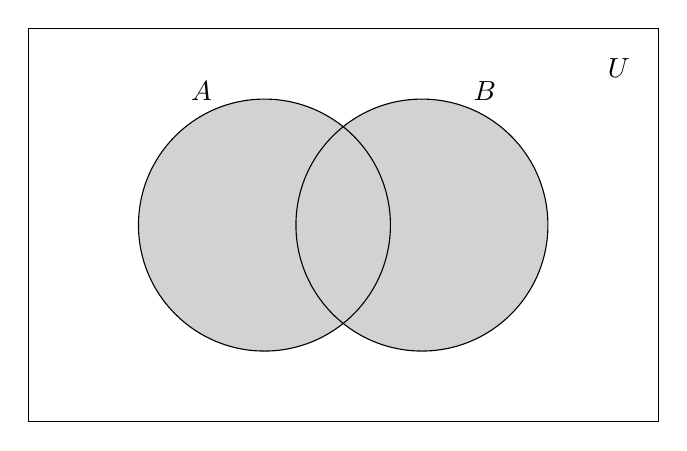
\begin{tikzpicture}

\draw (0,0) rectangle (8,5);
\node at (7.5,4.5) {$U$};

\fill[gray!35] (3,2.5) circle (1.6);
\fill[gray!35] (5,2.5) circle (1.6);

\draw (3,2.5) circle (1.6);
\draw (5,2.5) circle (1.6);

\node at (2.2,4.2) {$A$};
\node at (5.8,4.2) {$B$};

\end{tikzpicture}
\end{center}

The shaded region represents

\[
A\cup B.
\]

% -------------------------------------------------

\subsection{Intersection of Sets}

The intersection contains only those elements common to both sets.

It is denoted by

\[
A\cap B.
\]

Mathematically,

\[
A\cap B
=
\{x\mid x\in A\text{ and }x\in B\}.
\]

For the given sets,

\[
A\cap B=\{3,4\}.
\]

\subsubsection*{Venn Diagram}

\begin{center}
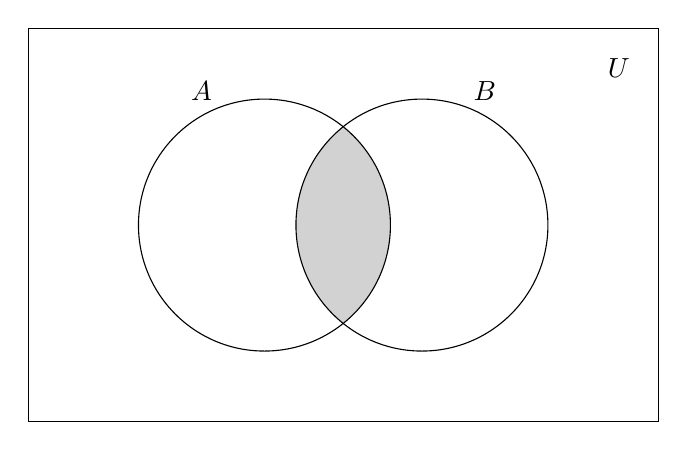
\begin{tikzpicture}

\draw (0,0) rectangle (8,5);
\node at (7.5,4.5) {$U$};

\begin{scope}
    \clip (3,2.5) circle (1.6);
    \fill[gray!35] (5,2.5) circle (1.6);
\end{scope}

\draw (3,2.5) circle (1.6);
\draw (5,2.5) circle (1.6);

\node at (2.2,4.2) {$A$};
\node at (5.8,4.2) {$B$};

\end{tikzpicture}
\end{center}

The shaded region represents

\[
A\cap B.
\]

% -------------------------------------------------

\subsection{Difference of Sets}

The difference of two sets contains the elements that belong to the first
set but do not belong to the second set.

It is denoted by

\[
A-B
\]

or

\[
A\setminus B.
\]

It is defined as

\[
A-B
=
\{x\mid x\in A\text{ and }x\notin B\}.
\]

For the given sets,

\[
A-B=\{1,2\}.
\]

Similarly,

\[
B-A=\{5,6\}.
\]

\subsubsection*{Venn Diagram for $A-B$}

\begin{center}
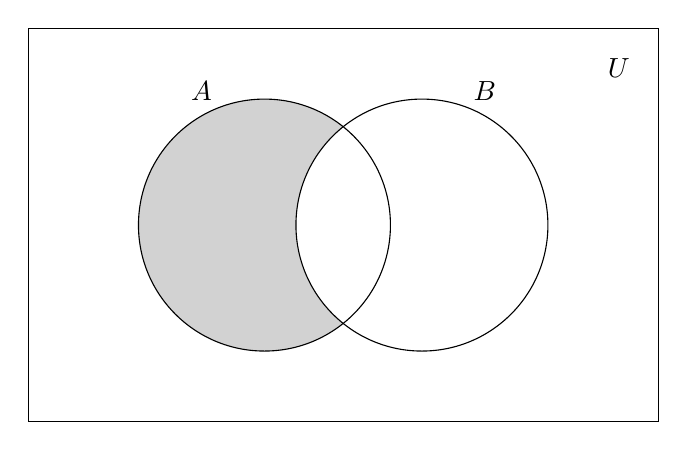
\begin{tikzpicture}

\draw (0,0) rectangle (8,5);
\node at (7.5,4.5) {$U$};

\fill[gray!35] (3,2.5) circle (1.6);

\begin{scope}
    \clip (5,2.5) circle (1.6);
    \fill[white] (3,2.5) circle (1.6);
\end{scope}

\draw (3,2.5) circle (1.6);
\draw (5,2.5) circle (1.6);

\node at (2.2,4.2) {$A$};
\node at (5.8,4.2) {$B$};

\end{tikzpicture}
\end{center}

The shaded region represents

\[
A-B.
\]

\subsubsection*{Venn Diagram for $B-A$}

\begin{center}
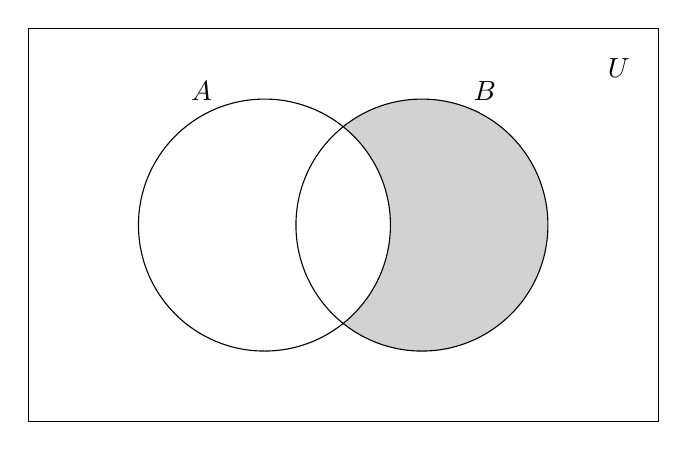
\begin{tikzpicture}

\draw (0,0) rectangle (8,5);
\node at (7.5,4.5) {$U$};

\fill[gray!35] (5,2.5) circle (1.6);

\begin{scope}
    \clip (3,2.5) circle (1.6);
    \fill[white] (5,2.5) circle (1.6);
\end{scope}

\draw (3,2.5) circle (1.6);
\draw (5,2.5) circle (1.6);

\node at (2.2,4.2) {$A$};
\node at (5.8,4.2) {$B$};

\end{tikzpicture}
\end{center}

The shaded region represents

\[
B-A.
\]

% -------------------------------------------------

\subsection{Symmetric Difference}

The symmetric difference contains the elements that belong to either $A$
or $B$, but not to both.

It is denoted by

\[
A\triangle B.
\]

It is defined as

\[
A\triangle B
=
(A-B)\cup(B-A).
\]

For the given sets,

\[
A-B=\{1,2\}
\]

and

\[
B-A=\{5,6\}.
\]

Therefore,

\[
A\triangle B=\{1,2,5,6\}.
\]

\subsubsection*{Venn Diagram}

\begin{center}
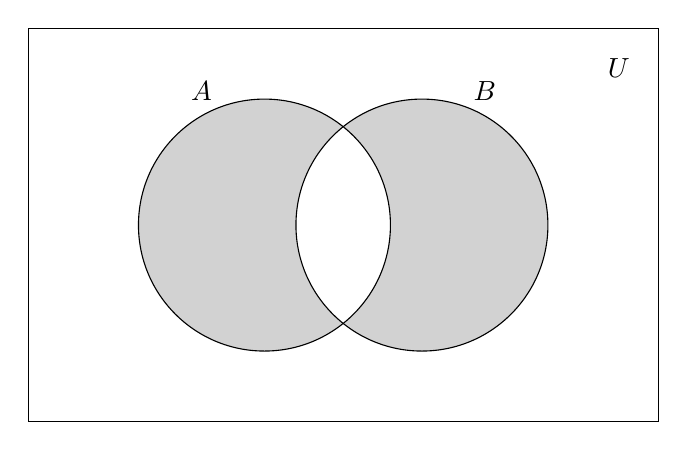
\begin{tikzpicture}

\draw (0,0) rectangle (8,5);
\node at (7.5,4.5) {$U$};

\fill[gray!35] (3,2.5) circle (1.6);
\fill[gray!35] (5,2.5) circle (1.6);

\begin{scope}
    \clip (3,2.5) circle (1.6);
    \fill[white] (5,2.5) circle (1.6);
\end{scope}

\draw (3,2.5) circle (1.6);
\draw (5,2.5) circle (1.6);

\node at (2.2,4.2) {$A$};
\node at (5.8,4.2) {$B$};

\end{tikzpicture}
\end{center}

The shaded regions represent

\[
A\triangle B.
\]

% -------------------------------------------------

\subsection{Complement of a Set}

The complement of a set consists of all elements in the universal set
that are not in the given set.

It is denoted by

\[
A^c
\]

or

\[
A'.
\]

The complement is defined as

\[
A^c=U-A.
\]

For example, let

\[
U=\{1,2,3,4,5,6,7,8\}
\]

and

\[
A=\{1,2,3,4\}.
\]

Then,

\[
A^c=\{5,6,7,8\}.
\]

\subsubsection*{Venn Diagram}

\begin{center}
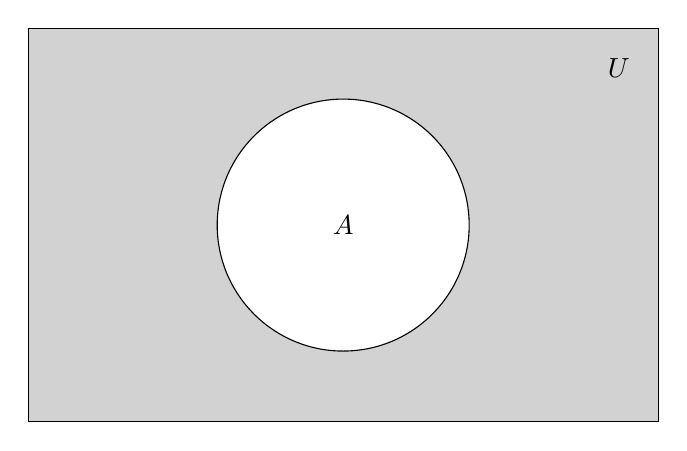
\begin{tikzpicture}

\draw[fill=gray!35] (0,0) rectangle (8,5);
\draw[fill=white] (4,2.5) circle (1.6);

\node at (7.5,4.5) {$U$};
\node at (4,2.5) {$A$};

\end{tikzpicture}
\end{center}

The shaded region represents

\[
A^c.
\]

% -------------------------------------------------

\subsection{Cartesian Product}

The Cartesian product of two sets is the set of all ordered pairs.

It is written as

\[
A\times B.
\]

It is defined as

\[
A\times B
=
\{(a,b)\mid a\in A,\ b\in B\}.
\]

For example, let

\[
A=\{1,2\}
\]

and

\[
B=\{x,y\}.
\]

Then

\[
A\times B
=
\{(1,x),(1,y),(2,x),(2,y)\}.
\]

Also,

\[
|A\times B|=|A|\times|B|.
\]

Therefore,

\[
|A\times B|=2\times2=4.
\]

% =================================================
% VENN DIAGRAMS
% =================================================

\section{Venn Diagrams}

A Venn diagram is a graphical representation of sets using closed curves,
usually circles. The universal set is represented by a rectangle.

For two sets $A$ and $B$, the main regions represented by Venn diagrams include

\begin{itemize}
    \item $A-B$: elements only in $A$.
    \item $B-A$: elements only in $B$.
    \item $A\cap B$: elements common to both sets.
    \item $A\cup B$: elements in at least one of the sets.
    \item $A\triangle B$: elements in exactly one of the sets.
    \item $A^c$: elements outside $A$ but inside the universal set.
\end{itemize}

Venn diagrams provide a visual way of understanding set operations.

% =================================================
% PRINCIPLE OF INCLUSION AND EXCLUSION
% =================================================

\section{Principle of Inclusion and Exclusion}

The Principle of Inclusion and Exclusion is used to determine the number
of elements in the union of two or more sets without counting common
elements more than once.

% -------------------------------------------------

\subsection{Formula for Two Sets}

For two finite sets $A$ and $B$,

\[
|A\cup B|
=
|A|+|B|-|A\cap B|.
\]

The intersection is subtracted because it is counted twice when $|A|$
and $|B|$ are added.

% -------------------------------------------------

\subsection{Formula for Three Sets}

For three sets $A$, $B$ and $C$,

\[
\begin{aligned}
|A\cup B\cup C|
={}&|A|+|B|+|C|\\
&-|A\cap B|-|A\cap C|-|B\cap C|\\
&+|A\cap B\cap C|.
\end{aligned}
\]

The pairwise intersections are subtracted because they are counted more
than once. The common intersection of all three sets is then added back.

% -------------------------------------------------

\subsection{Example}

Suppose

\[
|A|=20,\qquad
|B|=15,\qquad
|A\cap B|=5.
\]

Then,

\[
|A\cup B|
=
20+15-5
=
30.
\]

Hence, the union contains 30 elements.

% -------------------------------------------------

\subsection{Venn Diagram}

\begin{center}
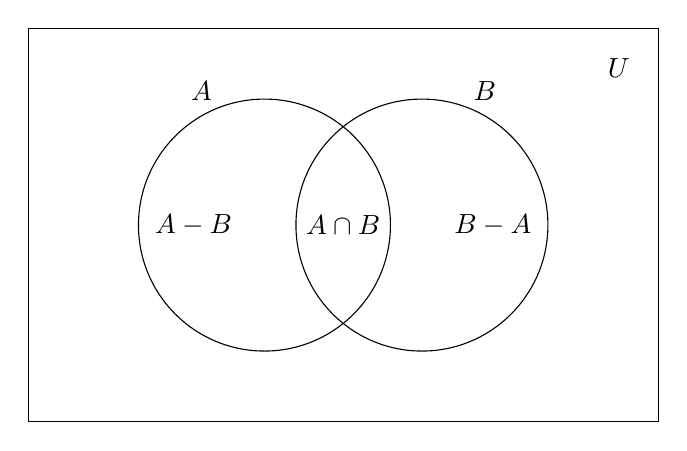
\begin{tikzpicture}

\draw (0,0) rectangle (8,5);
\node at (7.5,4.5) {$U$};

\draw (3,2.5) circle (1.6);
\draw (5,2.5) circle (1.6);

\node at (2.2,4.2) {$A$};
\node at (5.8,4.2) {$B$};

\node at (2.1,2.5) {$A-B$};
\node at (5.9,2.5) {$B-A$};
\node at (4,2.5) {$A\cap B$};

\end{tikzpicture}
\end{center}

% =================================================
% PARTIALLY ORDERED SETS
% =================================================

\section{Partially Ordered Sets (Posets)}

A partially ordered set, or \textbf{poset}, is a set together with a
relation that satisfies the following three properties:

\begin{enumerate}
    \item Reflexive
    \item Antisymmetric
    \item Transitive
\end{enumerate}

A poset is written as

\[
(P,\leq)
\]

where $P$ is the set and $\leq$ is the partial order.

% -------------------------------------------------

\subsection{Reflexive Property}

A relation is reflexive if

\[
a\leq a
\]

for every $a\in P$.

% -------------------------------------------------

\subsection{Antisymmetric Property}

A relation is antisymmetric if

\[
a\leq b
\quad\text{and}\quad
b\leq a
\]

implies

\[
a=b.
\]

% -------------------------------------------------

\subsection{Transitive Property}

A relation is transitive if

\[
a\leq b
\quad\text{and}\quad
b\leq c
\]

implies

\[
a\leq c.
\]

% -------------------------------------------------

\subsection{Example}

Consider the power set

\[
\mathcal{P}(\{a,b\})
=
\{\emptyset,\{a\},\{b\},\{a,b\}\}
\]

with the subset relation $\subseteq$.

Thus,

\[
(\mathcal{P}(\{a,b\}),\subseteq)
\]

forms a partially ordered set.

For example,

\[
\emptyset\subseteq\{a\},
\]

\[
\emptyset\subseteq\{b\},
\]

\[
\{a\}\subseteq\{a,b\},
\]

and

\[
\{b\}\subseteq\{a,b\}.
\]

% =================================================
% HASSE DIAGRAM
% =================================================

\section{Hasse Diagram}

A Hasse diagram is a simplified graphical representation of a finite
partially ordered set.

In a Hasse diagram:

\begin{itemize}
    \item Reflexive relations are not shown.
    \item Transitive relations are not shown directly.
    \item Only immediate ordering relations are represented by lines.
\end{itemize}

For the power set

\[
\mathcal{P}(\{a,b\})
=
\{\emptyset,\{a\},\{b\},\{a,b\}\},
\]

under the subset relation $\subseteq$, the Hasse diagram is shown below.

\begin{center}

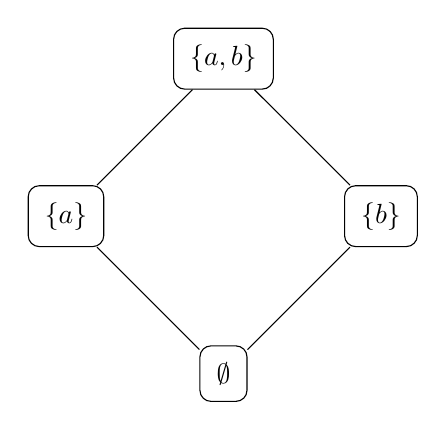
\begin{tikzpicture}[
    every node/.style={
        draw,
        rounded corners,
        inner sep=6pt
    }
]

\node (top) at (0,4) {$\{a,b\}$};

\node (a) at (-2,2) {$\{a\}$};
\node (b) at (2,2) {$\{b\}$};

\node (bottom) at (0,0) {$\emptyset$};

\draw (bottom)--(a);
\draw (bottom)--(b);
\draw (a)--(top);
\draw (b)--(top);

\end{tikzpicture}

\end{center}

The empty set is the smallest element, while $\{a,b\}$ is the largest
element.

The diagram represents

\[
\emptyset\subset\{a\}\subset\{a,b\}
\]

and

\[
\emptyset\subset\{b\}\subset\{a,b\}.
\]

Thus, a Hasse diagram provides a compact representation of the ordering
between the subsets.

% =================================================
% USEFUL CARDINALITY RESULTS
% =================================================

\section{Useful Cardinality Results}

For finite sets $A$ and $B$,

\[
|A\cup B|
=
|A|+|B|-|A\cap B|.
\]

If $A$ and $B$ are disjoint, then

\[
A\cap B=\emptyset
\]

and therefore

\[
|A\cup B|=|A|+|B|.
\]

For the power set,

\[
|\mathcal{P}(A)|=2^{|A|}.
\]

For the Cartesian product,

\[
|A\times B|=|A||B|.
\]

For example, if

\[
|A|=3,
\]

then

\[
|\mathcal{P}(A)|=2^3=8.
\]

If

\[
|A|=3
\quad\text{and}\quad
|B|=4,
\]

then

\[
|A\times B|=3\times4=12.
\]

% =================================================
% CONCLUSION
% =================================================

\section{Conclusion}

Set theory provides the basic framework for describing collections of
objects and the relationships between them. Important concepts include
different types of sets, cardinality, set-builder form, subsets, power
sets and countability.

Set operations such as union, intersection, difference, symmetric
difference, complement and Cartesian product are useful in many areas
of mathematics and computer science. Venn diagrams provide a visual
representation of these operations.

The power set under the subset relation forms a partially ordered set,
which can be represented using a Hasse diagram. These concepts provide
an important foundation for further topics in mathematics and computer
science.

\vspace{1cm}

\begin{center}
\textbf{--- End ---}
\end{center}

\end{document}